\chapter{\babDua}
Membuat desain sebuah perangkat IC membutuhkan proses yang panjang dan sumberdaya manusia yang banyak, serta tingkat ketelitian yang tinggi. Oleh karenanya di butuhkan biaya yang tidak kecil dan waktu yang cukup lama hanya untuk membuat sebuah desain IC. Dengan kerumitan yang tinggi serta waktu yang lama dalam setiap prosesnya kadang pihak yang tak bertanggung jawab melakukan kecurangna dengan mecuri desain untuk memotong waktu dan biaya yang di butuhkan utuk produksi. sehingga menjadi masalah dalam dunia permanufakturan ic. \cite{Azriel2017}

\section{Very Large Scale Integration}
\textit{Very Large Scale Integration} atau disingkat LSI merupakan proses pembuatan sebuah IC dengan mengkombinasikan ribuan transistor ke dalam sebuah chip. VLSI ada sejak tahun 1970-an ketika semikonduktor kompleks dan teknologi komunikasi sedang berkembang. Mikroprosesor merupakan salah satu peraangkat VLSI. Sebelum adanya teknologi VLSI kebanyakan IC memiliki set fungsi yang terbatas yang dapat di jalankan. Sebuah perangkat chip elektronik dahulu hanya fokus pada sebuah fungsi seperti CPU, ROM, RAM dan rangkaian logika lainnya. Dengan adanya VLSI memungkinkan disainer IC untuk menambahkan berbagai fungsi kedalam sebuah chip IC. \cite{vlsi.hist} 

\subsection{Arus Pengembangan LSI}
Integrated Circuit (IC) merupakan teknologi sirkuit elektronika yang lebih maju. Sebuah rangkaian elektronika dibuat dari berbagai komponen elektronika yang berbeda beda seperti transistor, resistor, kapasitor dan dioda yang saling tersambung satu sama lain. \cite{vlsi.hist}

Transistor merupakan komponen terpenting pada pengembangan teknologi komputer moderen. Sebelum ditemukannya transistor. Para Engineer harus menggunakan tabung vakum. Tabung vakum dapat bekerja sebagai saklar elektronik. Namun tabung vakum membutuhkan daya dan ruang yang besar, mahal, serta kemampuan eksekusi yang lambat membuat tabung vakum tergantikan oleh transistor.

Dengan ditemukannya transistor yang ukuran dan kebutuhan dayanya yang kecil namun tetap efektif, Para Engineer elektronik di tahun 1950an melihat banyak sekali kemungkinan untuk implementasinya pada rangkaian elektronik yang lebih maju. Dengan semakin meningkatnya kompleksitas pada rangkaian elektronik munculah masalah-masalah baru.

Salah satunya adalah ukuran rangkaian. Sebuah rangkaian kompleks seperti komputer sangat bergantung pada kecepatan. Apabila jumlah komponen pada komputer terlalu banyak maka sambungan antar komponen juga semakin banyak dan semakin panjang, sehingga menyebabkan kecepatan transfer sinyal listrik menjadi berkurang yang menyebabkan proses pada komputer menjadi lambat.

Tahun 1958 masalah ini dapat dipecahkan oleh ide Jack S Kilby yang idenya adalah merangkai komponen elektronika dalam sebuah blok silikon (Monolithic Idea). Idenya tersebut tidak hanya mengurangi ukuran rangkaian namun juga mengurangi kebutuhan kabel sambungan antar rangkaian serta manufakturingnya dapat diautomasi. Akan tetapi idenya tersebut masih memiliki banyak masalah lain. Walaupun begitu, idenya tersebut mendapatkan penghargaan nobel di tahun 2000.

Setengah tahun setelah Kilby mencetuskan idenya tentang rangkaian Monolithic. Robert Noyce memiliki jawaban untuk beberapa permasalahan pada ide Kilby. Yaitu interkoneksi antar rangkaian. Yaitu menambahkan lapisan metal pada lapisan terakhir dan menghilangkan sebagian lapisannya sehingga sambungan antar komponen dapat terbentuk.

\begin{figure}
	\centering
	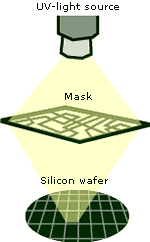
\includegraphics[width=0.35\textwidth]
	{pics/steping.png}
	\caption{Produksi Chip Moderen}
	\label{fig:produksiChipModeren}
\end{figure}

Chip pada zaman sekarang berbasis pada photolithography. Pada teknik ini digunakan radiasi sinar Ultra Violet yang melewati sebuah mask menuju lembaran silikon yang di lapisi filem photosensitive untuk membentuk suatu rangkaian.

\subsection{Kemungkinan Serangan Desain LSI}
Terdapat banyak kemungkinan serangan dalam proses manufakturing desain LSI. Berikut beberapa contoh serangan terhadap LSI desain.

\begin{figure}
	\centering
	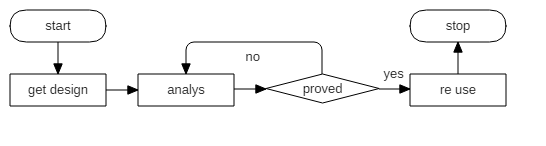
\includegraphics[width=1.05\textwidth]
	{diagrams/untrustSource.png}
	\caption{Clonning/Sumber Tidak Terpercaya}
	\label{fig:untrustsource}
\end{figure}

Dalam segi ini serangan dilakukan dengan cara mencuri langsung desain yang sudah siap di fabrikasi serta uji coba kebenaran. Bila pencuri mendapatkan desain yang telah di uji coba, maka pencuri tinggal langsung memperbanyak desain yang telah di curi.

\begin{figure}
	\centering
	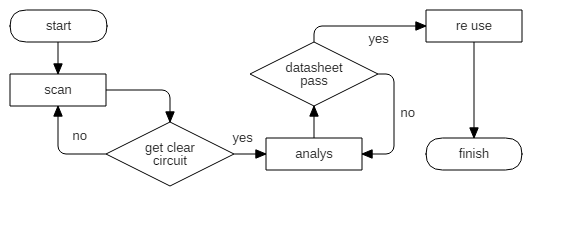
\includegraphics[width=1.05\textwidth]
	{diagrams/reverseEngineering.png}
	\caption{RE (Reverse Engineering)}
	\label{fig:reverseengineering}
\end{figure}

Untuk serangan jenis ini, pencuri sudah pendapatkan produk dari pasar yang telah teruji, pencuri tinggal melakukan scan rangkaian kemudian mengujinya dengan datasheet. Apabila hasil scan desain produk di dapati rangkaian yang konkrit/jelas dan rangkaian tersebut telah teruji sesuai datasheet. Maka pencuri tinggal melakukan fabrikasi.

\subsection{Mengatasi Serangan terhadap Desain LSI}
Dengan meninjau kemungkinan dari tipe serangan, terdapat berbagai cara untuk mengatasi setiap serangan serangan tersebut. Dari reverse engineering hingga untrust source. untuk reverse enginering digunakan teknik anti reverse engineering dan untuk untrust source digunakan teknik identifier dan dengan enclosure agreement law.

\begin{figure}
	\centering
	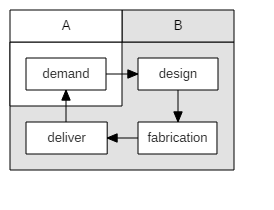
\includegraphics[width=0.6\textwidth]
	{diagrams/oldBusinessLSI.png}
	\caption{Model Bisnis Lama}
	\label{fig:oldbiss}
\end{figure}

\begin{figure}
	\centering
	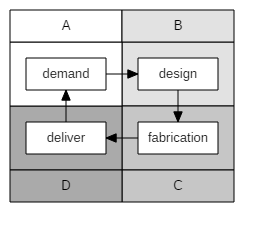
\includegraphics[width=0.6\textwidth]
	{diagrams/newBusinessLSI.png}
	\caption{Model Bisnis Baru}
	\label{fig:newbiss}
\end{figure}

\section{Teknik Proteksi}
Dari berbagai teknik yang telah digunakan, penulis melakukan penggabungan 2 teknik pengamanan dalam sebuah desain IC. Dalam penelitian ini dilakukan penggabungan 2 teknik agar cakupan wilayah keamanan sebuah IC semakin luas. Berikut teknik yang digabungkan dalam penelitian kali ini.

\subsection{DSP (Digital Signal Processing) Filter}
DSP merupakan teknik pengolahan sinyal untuk sinyal digital.

\subsection{Polimorphisme}
Polimorphisme merupakan teknik pengecoh yang di gunakan dalam perlindungan desain IC. 

\begin{figure}
	\centering
	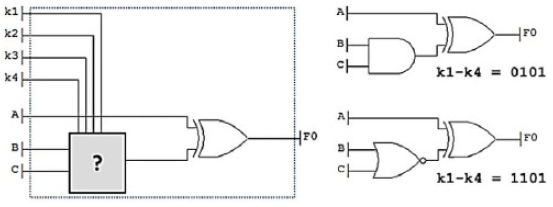
\includegraphics[width=0.75\textwidth]
	{pics/polymorphgate.png}
	\caption{Polymorph gate}
	\label{fig:poly}
\end{figure}

\section{Peralatan dan Teknologi}
Dalam penelitian kali ini dibutuhkan beberapa peralatan dan standard teknologi untuk mengembangkan teknik perlindungan intelektual properti. Sebagai penunjang dalam pembuatan perlindungan, penulis menggunakan tools dan teknologi yang umum digunakan dalam proses pengembangan desain LSI.

\subsection{Verilog HDL}
Verilog HDL merupakan bahasa pendeskripsi hardware yang di rancang untuk mendeskripsikan suatu rancangan perangkat keras pada gate-lavel dalam bentuk bahasa manusia *walaupun enggak begitu manusiawi

\subsection{YOSYS}
YOSYS adalaha...

\subsection{FPGA Elbert V2 Board}
FPGA merupakan kepanjangan dari Field Programmable Gate Array adalah perangkat keras yang biasa digunakan dalam proses manufakturing IC. FPGA digunakan untuk mensimulasikan draft rancangan IC yang siap untuk di test yang apabila telah lolos test akan di lanjutkan ke tahap layout. FPGA hanya digunakan apabila rancangan membutuhkan input dari perangkat lain atau program kernel.

\section{Target IP Core}
Watermark adalah rangkaian yang tidak dapat berdiri sendiri pada implementasinya walaupun dalam pengembangannya bisa di lakukan mandiri. Watermark dalam bentuk data signature.

\subsection{ALU (Aritmatic Logic Unit)}
Aritmatik Logic Unit atau dapat di singkat sebagai ALU merupakan salah satu komponen utama dalam prosesor. ALU berfungsi sebagai Unit yang melakukan kalkulasi logika artimatika.
